% GENERATED by scripts/generate-paper-figures.ts from
% data/reports/baselines-report.json — do not edit by hand.
\begin{figure*}[t]
\centering
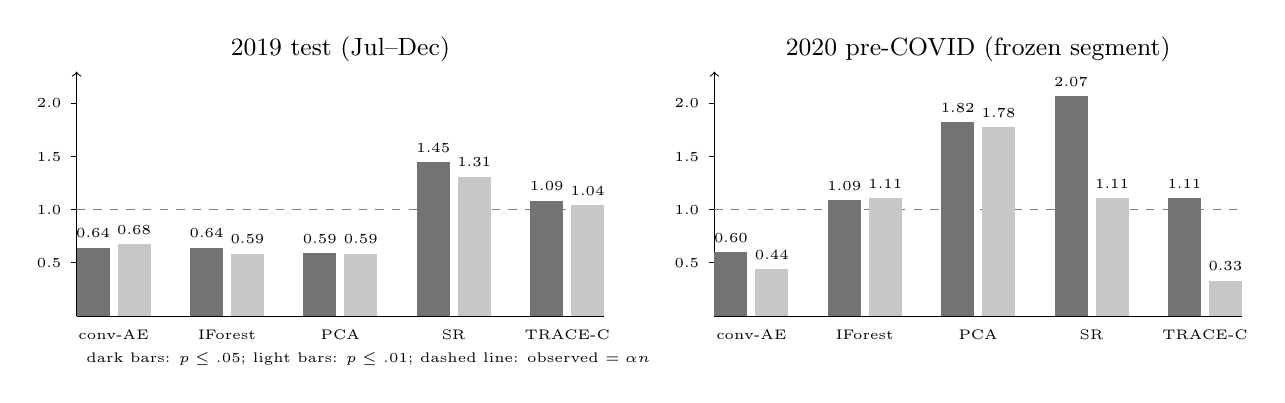
\begin{tikzpicture}
% panel: 2019 test (Jul--Dec)
\draw[->] (0,0) -- (0,3.105);
\draw (0,0) -- (6.700,0);
\draw (0,0.675) -- (-0.07,0.675) node[left,font=\tiny] {0.5};
\draw (0,1.350) -- (-0.07,1.350) node[left,font=\tiny] {1.0};
\draw (0,2.025) -- (-0.07,2.025) node[left,font=\tiny] {1.5};
\draw (0,2.700) -- (-0.07,2.700) node[left,font=\tiny] {2.0};
\draw[dashed,gray] (0,1.350) -- (6.700,1.350);
\fill[black!55] (0.000,0) rectangle (0.420,0.868);
\node[above,font=\tiny] at (0.210,0.868) {0.64};
\fill[black!22] (0.520,0) rectangle (0.940,0.916);
\node[above,font=\tiny] at (0.730,0.916) {0.68};
\node[below,font=\tiny] at (0.470,-0.06) {conv-AE};
\fill[black!55] (1.440,0) rectangle (1.860,0.868);
\node[above,font=\tiny] at (1.650,0.868) {0.64};
\fill[black!22] (1.960,0) rectangle (2.380,0.794);
\node[above,font=\tiny] at (2.170,0.794) {0.59};
\node[below,font=\tiny] at (1.910,-0.06) {IForest};
\fill[black!55] (2.880,0) rectangle (3.300,0.795);
\node[above,font=\tiny] at (3.090,0.795) {0.59};
\fill[black!22] (3.400,0) rectangle (3.820,0.794);
\node[above,font=\tiny] at (3.610,0.794) {0.59};
\node[below,font=\tiny] at (3.350,-0.06) {PCA};
\fill[black!55] (4.320,0) rectangle (4.740,1.957);
\node[above,font=\tiny] at (4.530,1.957) {1.45};
\fill[black!22] (4.840,0) rectangle (5.260,1.771);
\node[above,font=\tiny] at (5.050,1.771) {1.31};
\node[below,font=\tiny] at (4.790,-0.06) {SR};
\fill[black!55] (5.760,0) rectangle (6.180,1.467);
\node[above,font=\tiny] at (5.970,1.467) {1.09};
\fill[black!22] (6.280,0) rectangle (6.700,1.405);
\node[above,font=\tiny] at (6.490,1.405) {1.04};
\node[below,font=\tiny] at (6.230,-0.06) {TRACE-C};
\node[above,font=\small] at (3.350,3.105) {2019 test (Jul--Dec)};
\begin{scope}[xshift=8.100cm]
% panel: 2020 pre-COVID (frozen segment)
\draw[->] (0,0) -- (0,3.105);
\draw (0,0) -- (6.700,0);
\draw (0,0.675) -- (-0.07,0.675) node[left,font=\tiny] {0.5};
\draw (0,1.350) -- (-0.07,1.350) node[left,font=\tiny] {1.0};
\draw (0,2.025) -- (-0.07,2.025) node[left,font=\tiny] {1.5};
\draw (0,2.700) -- (-0.07,2.700) node[left,font=\tiny] {2.0};
\draw[dashed,gray] (0,1.350) -- (6.700,1.350);
\fill[black!55] (0.000,0) rectangle (0.420,0.810);
\node[above,font=\tiny] at (0.210,0.810) {0.60};
\fill[black!22] (0.520,0) rectangle (0.940,0.600);
\node[above,font=\tiny] at (0.730,0.600) {0.44};
\node[below,font=\tiny] at (0.470,-0.06) {conv-AE};
\fill[black!55] (1.440,0) rectangle (1.860,1.470);
\node[above,font=\tiny] at (1.650,1.470) {1.09};
\fill[black!22] (1.960,0) rectangle (2.380,1.500);
\node[above,font=\tiny] at (2.170,1.500) {1.11};
\node[below,font=\tiny] at (1.910,-0.06) {IForest};
\fill[black!55] (2.880,0) rectangle (3.300,2.460);
\node[above,font=\tiny] at (3.090,2.460) {1.82};
\fill[black!22] (3.400,0) rectangle (3.820,2.400);
\node[above,font=\tiny] at (3.610,2.400) {1.78};
\node[below,font=\tiny] at (3.350,-0.06) {PCA};
\fill[black!55] (4.320,0) rectangle (4.740,2.790);
\node[above,font=\tiny] at (4.530,2.790) {2.07};
\fill[black!22] (4.840,0) rectangle (5.260,1.500);
\node[above,font=\tiny] at (5.050,1.500) {1.11};
\node[below,font=\tiny] at (4.790,-0.06) {SR};
\fill[black!55] (5.760,0) rectangle (6.180,1.500);
\node[above,font=\tiny] at (5.970,1.500) {1.11};
\fill[black!22] (6.280,0) rectangle (6.700,0.450);
\node[above,font=\tiny] at (6.490,0.450) {0.33};
\node[below,font=\tiny] at (6.230,-0.06) {TRACE-C};
\node[above,font=\small] at (3.350,3.105) {2020 pre-COVID (frozen segment)};
\end{scope}
\node[font=\tiny,anchor=west] at (0,-0.55)
  {dark bars: $p\leq.05$; light bars: $p\leq.01$; dashed line: observed $=\alpha n$};
\end{tikzpicture}
\caption{Empirical rank diagnostics under the shared scoring envelope:
observed counts of outer rank values at thresholds $.05$ and $.01$, expressed
as a ratio to the arithmetic benchmark $\alpha n$ (dashed line). Values are
read directly from the committed reports. Descriptive only: autocorrelation,
drift, reused references, and known events preclude reading these as uniform
$p$-value or false-discovery guarantees (Section~\ref{sec:results}).}
\label{fig:rank-diagnostics}
\end{figure*}
